%4.1.tex

LLVMにおいて特定のターゲットマシン命令の生成は\ref{chp:3_1}で述べたSelectionDAGISelパスによるSelectフェーズにてLLVM IRの命令からターゲットマシン命令に変換されることによって行われる.
この変換はSelectionDAGのノードに対してパターンマッチングを行い,特定のパターンにターゲット命令を対応させる手法で行われる.

このパターンマッチングに用いるパターン記述はLLVMの固有ドメイン言語であるTableGenによって行われる.TableGenはアセンブリコードやオブジェクトファイルの生成対象であるアーキテクチャであるターゲットマシンで定義されている命令やレジスタ等の情報を記述することに特化しているドメイン固有言語である.TableGenでは命令コード生成のためにパターンの定義だけでなく,アセンブリコードやオブジェクトファイルの出力のために命令ニーモニックの定義や命令フォーマットの定義も行っている.

SelectionDAGのパターンマッチングの例を図\ref{fig:SelectionDAG_example}
に示す.
図\ref{fig:SelectionDAG_example}
では加算命令の例を示している.図\ref{fig:SelectionDAG_example}の上部にパターン定義クラスPatが記述されている.Patクラスの第一引数と変換前のSelectionDAGのノードが一致した場合,Patクラスの第二引数で指定したノードに変換する.

\begin{figure}[bt]
    \centering
    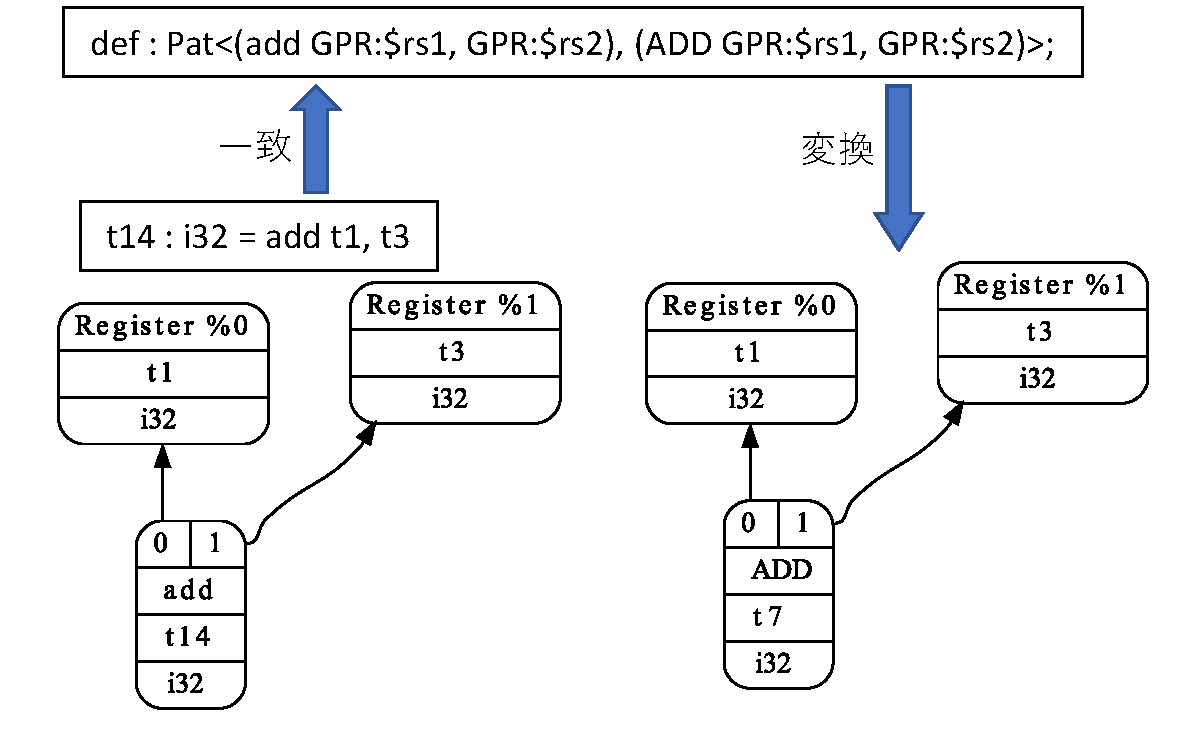
\includegraphics[scale=0.6]{image/SelectionDAG_example.pdf}
    \caption{SelectionDAGの命令変換}
    \label{fig:SelectionDAG_example}
\end{figure}

この様にSelectionDAGのパターンと命令ごとに定義されているパターンが一致したときに対応した命令にノードが変換される.
LLVMのバージョン13.0.0ではRISC-Vのベクトル命令のためのパターン定義が既に実装されており,そのパターンと一致した際に変換する命令を独自のベクトル拡張付きRISC-Vの命令コードに定義しなおすことによってベクトル拡張付きRISC-V命令の生成を実現する.

LLVMにおける命令の定義は命令フォーマットの定義と命令ニーモニックの定義に分かれる.命令フォーマットの定義はTableGenによって命令の種類ごとに命令フォーマットのクラス定義を行う.LLVMにおけるRISC-Vの命令フォーマットは基本クラスであるクラスRVInstを継承する形で行われる.RVInstでは32ビットの命令フィールドを格納するInstや命令のニーモニックを格納するAsmStringが定義されている.LLVMではこのRVInstを継承してInstの命令フィールドの定義や命令のニーモニックをAsmStringに格納する形で定義することで異なる命令フォーマットの定義を行う.

命令ニーモニックの定義は命令フォーマットを定義したクラスを継承して入出力レジスタの定義を行ったクラスをインスタンス化する際に行う.入出力レジスタを定義するクラスは似たような入出力レジスタを持つ命令を定義する場合において同じ入出力レジスタの定義を何度も繰り返さないために定義を行う.

命令フォーマット,命令ニーモニック定義のクラスの継承関係を図\ref{fig:InstFromat_class}
に示す.基本クラスであるRVInstを継承して基本命令のフォーマットの定義を行っている.クラスALU\_rr,ALU\_riはそれぞれ算術演算命令のためのクラスである.ALU\_rrは汎用レジスタ同士の加算や減算の算術演算の定義に用いられ,ALU\_riは即値を用いた算術演算の命令定義に用いられる.

\begin{figure}[tb]
    \centering
    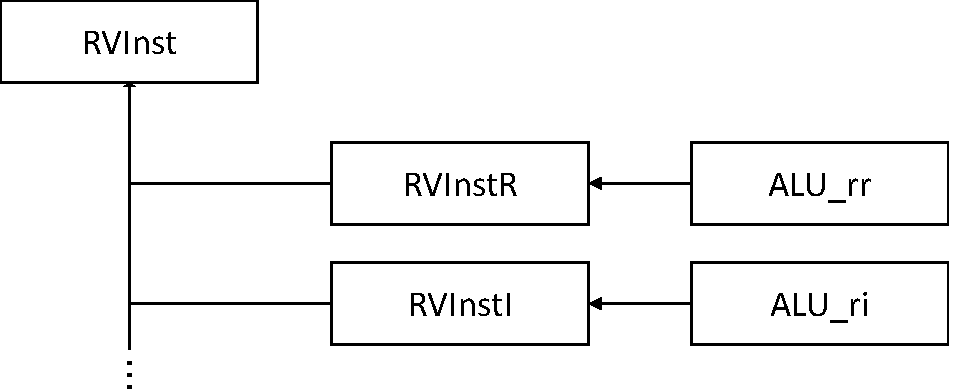
\includegraphics[scale=0.5]{image/InstFormat_class.pdf}
    \caption{基本命令フォーマットクラス継承関係}
    \label{fig:InstFromat_class}
\end{figure}

LLVMでは上記のように命令ニーモニックの定義が行われており,この定義方法に従った形式でベクトル拡張付きRISC-Vのベクトル命令の定義を行う.